\documentclass{standalone}
\usepackage{amssymb} % мат. символы
    \DeclareMathSymbol{\sm}{\mathbin}{AMSa}{"39} % короткий минус

\usepackage{tikz}
    \usetikzlibrary{arrows.meta}
    \usetikzlibrary{calc}

\tikzset{gdst/.style=
    {circle, draw=black!50, very thick, minimum height=1.2cm, inner sep=2pt, text centered, }, }
    
\begin{document}
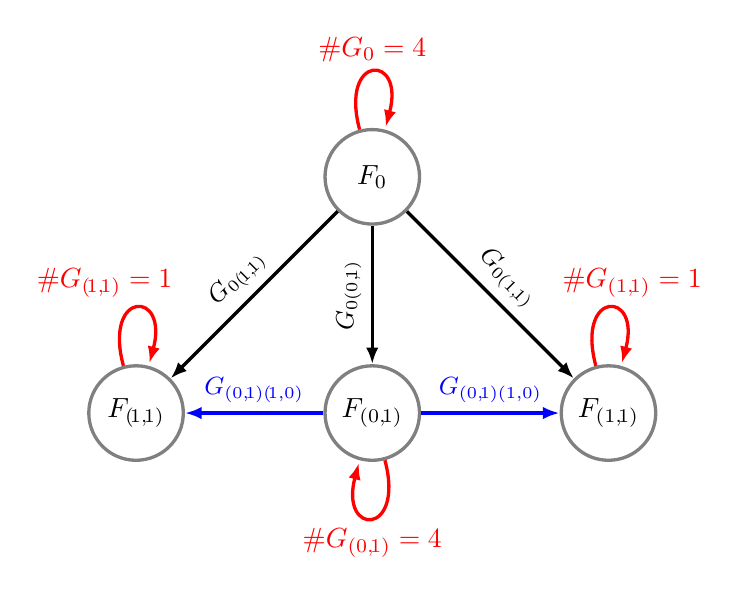
\begin{tikzpicture}
    \node[gdst, shift={(0,0)}] (f1){$F_{(\sm\!1,\sm\!1)}$};
    \node[gdst, shift={(3,0)}] (f2){$F_{(0,\sm\!1)}$};
    \node[gdst, shift={(6,0)}] (f3){$F_{(1,\sm\!1)}$};
    \node[gdst, shift={(3,3)}] (f5){$F_{0}$};
    \path[<-,>={Latex[length=6pt]}, very thick] 
        (f1) edge[blue] node[above] {\small$G_{(0,\sm\!1)(\sm\!1,0)}$} (f2)
             edge node[above, rotate=45] {\small$G_{0(\sm\!1,\sm\!1)}$} (f5) 
             edge[loop above, red] node[above, shift={(-0.4,0)}] {$\#G_{(\sm\!1,\sm\!1)}=1$} (f1)
        (f3) edge[blue] node[above] {\small$G_{(0,\sm\!1)(1,0)}$} (f2)  
             edge node[above, rotate=-45] {\small$G_{0(1,\sm\!1)}$} (f5)
             edge[loop above, red] node[above, shift={(0.3,0)}] {$\#G_{(1,\sm\!1)}=1$} (f3)
        (f2) edge node[above, rotate=90] {\small$G_{0(0,\sm\!1)}$} (f5)
             edge[loop below, red] node[below] {$\#G_{(0,\sm\!1)}=4$} (f2)
        (f5) edge[loop above, red] node[above] {$\# G_{0}=4$} (f5);
\end{tikzpicture}
\end{document}